\subsection[Przegląd protokołów wykorzystywanych w IoT]{Przegląd protokołów wykorzystywanych w IoT}
\begin{itemize}
    \item Message Queue Telemetry Transport (MQTT) jest lekkim protokołem transmisji danych, umożliwia komunikację między systemami za pośrednictwem serwera. MQTT jest oparty o wzorzec Publish-Subscribe, wzorzec ten mówi, że wiadomość od nadawcy nie trafia bezpośrednio do odbiorcy tylko najpierw trafia do serwera pośredniczącego (ang. broker). Dzięki serwerowi pośredniczącemu odbiorca nic nie wie o osobie która nadaj wiadomość oraz nie dostaje potwierdzenia o doręczonej wiadomości. %//tutaj trzebaz zmienić jeśli dodam Qos.
    Plusami protokołu MQTT jest na pewno prędkość przesyłania danych, zawdzięcza to dzięki małemu narzutowi na transportowane dane. Narzut na dane oznacza, ile jest potrzebnych dodatkowych bajtów przy wysłaniu wiadomości, najmniejszy pakiet (przy zastosowaniu MQTT) ma tylko dwa bajty metadanych. Jest to również protokół binarny, co wpływa na zmniejszenie obciążenia. Dodatkowo zapewnia bardzo wysoką niezawodność transmisji, dlatego idealnie sprawdza się przy połączeniach między dwoma urządzeniami. Kolejną zaletą protokołu MQTT jest możliwość komunikacji dwukierunkowej oznacza to, że klient MQTT może być równocześnie subskrybentem jak i publisherem. %// można jeszcze dodać coś o możliwość zarządzania jakością usług ale tego nie robiliśmy więc nwm czy wspominać ??
\end{itemize}
\begin{figure}[H]
    \centering
    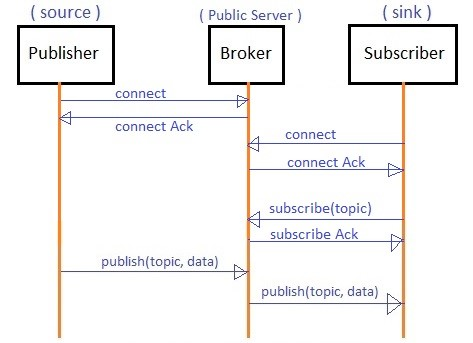
\includegraphics[width=\textwidth]{kp07}
    \caption{Diagram przesyłania wiadomości w protokole MQTT} %publish/subscribe
    \label{fig:iotarch1}
\end{figure}
\begin{itemize}
    \item WebSocket jest protokołem opartym na TCP, tak jak MQTT zapewnia komunikację dwukierunkową. Po zestawieniu połączenia zarówno serwer jak i urządzenie mogą w dowolnym momencie wymieniać się danymi. WebSocket jest dużo lepszym rozwiązaniem od np. AJAX long polling (rozwiązanie, gdzie klient wysyła żądanie a serwer odpowiada), ponieważ mogą obsłużyć w tym samym czasie większą ilość zapytań. Minusem tego rozwiązania jest duży narzut danych, wynikający z złożoności ramek.
\end{itemize}
\begin{figure}[H]
    \centering
    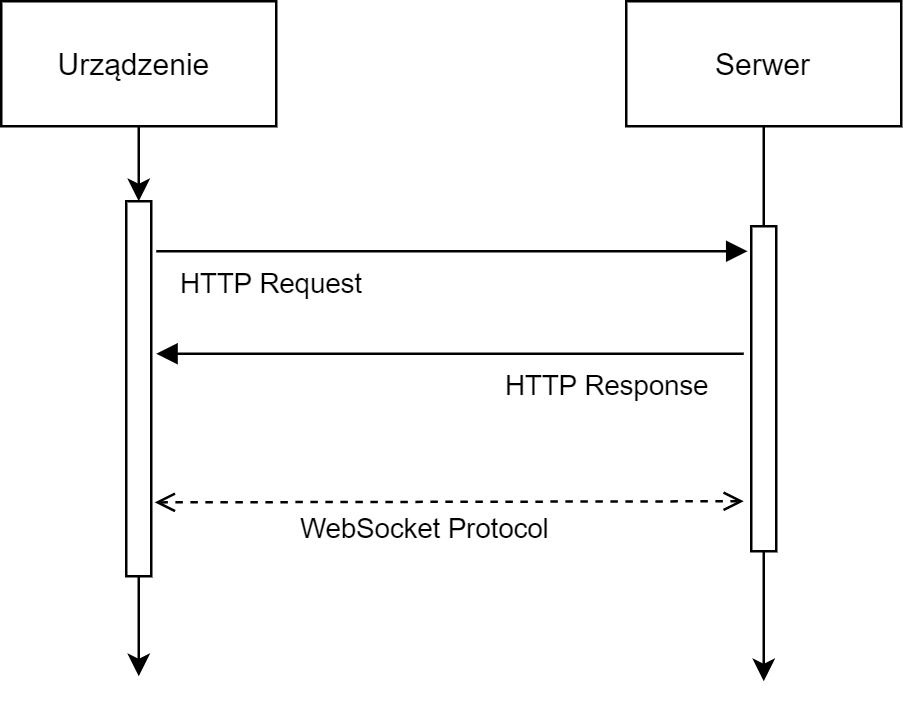
\includegraphics[width=\textwidth]{kp05}
    \caption{Diagram ukazujący jak działa Websocket}
    \label{fig:iotarch2}
\end{figure}
\begin{itemize}
    \item Constrained Application Protocol (CoAP) to protokół warstwy aplikacji, który jest stosowany do urządzeń z ograniczonymi zasobami. CoAP jest oparty na UDP a nie TCP, dlatego klient komunikuje się bezpołączeniowo z serwerem za pośrednictwem pakietów. Umożliwia również komunikowanie się za pomocą podobnych protokołów oraz obsługuje multiemisjie. CoAP został zaprojektowany do komunikacji między urządzeniami znajdującymi się w tej samej ograniczonej sieci.
\end{itemize}
\begin{figure}[H]
    \centering
    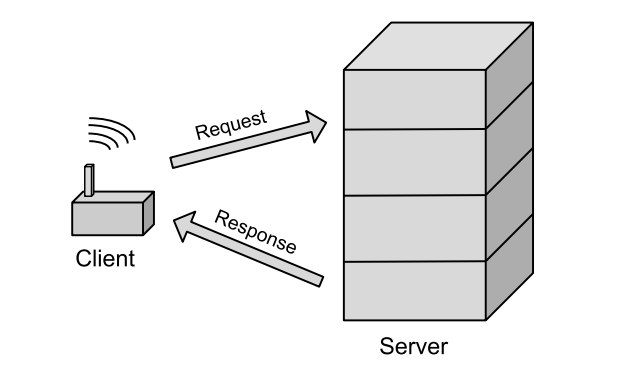
\includegraphics[width=\textwidth]{kp06.png}
    \caption{Schemat pokazujący sposób komunikacji w protokole CoAP}
    \label{fig:iotarch3}
\end{figure}
\begin{itemize}
    \item Hypertext Transfer Protocol (HTTP) to protokół warstwy aplikacji, który służy do przesyłania dokumentów hipermedialnych. HTTP jest oparty o wzorzec klient-serwer, gdzie klient (lub serwer proxy w jego imieniu) wysyła żądanie, a następnie czeka na odpowiedz. Protokół HTTP jest bezstanowy, oznacza to, że nie zawiera żadnych danych o połączeniu. Najczęściej jest oparty na warstwie TCP / IP, może być również na dowolnej niezawodnej warstwie transportowej.
\end{itemize}
\begin{figure}[H]
    \centering
    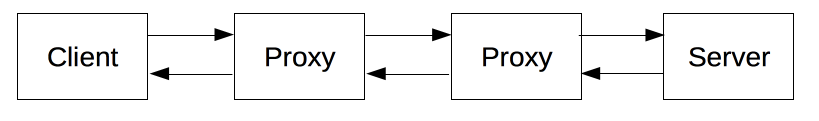
\includegraphics[width=\textwidth]{kp08.png}
    \caption{Wykorzystanie serwerów proxy w komunikacji}
    \label{fig:iotarch4}
\end{figure}
//dodać do literatury https://www.czasopismologistyka.pl/artykuly-naukowe/send/333-artykuly-na-plycie-cd-1/7760-kazala-wykorzystanie-protokolu
% dodać do literatury https://www.net.in.tum.de/fileadmin/TUM/NET/NET-2018-03-1/NET-2018-03-1_02.pdf
% //jesli dodam tabele to tez to http://stephendnicholas.com/posts/power-profiling-mqtt-vs-https
//być może jescze to można dodać https://www.controlengineering.pl/wp-content/uploads/2018/07/Fabryka-4.0-CE.pdf
